 
\documentclass[12pt]{article}
 %author David Dobor
\usepackage[margin=1in]{geometry} 
\usepackage{amsmath,amsthm,amssymb}
 \usepackage{graphicx}
\usepackage[scaled]{helvet}
\usepackage{hyperref}
\usepackage[usenames,dvipsnames,svgnames,table]{xcolor}
\usepackage[T1]{fontenc}
\usepackage{palatino}
%\renewcommand*\familydefault{\sfdefault} %% Only if the base font of the document is to be sans serif

\newcommand{\N}{\mathbb{N}}
\newcommand{\Z}{\mathbb{Z}}


\newcommand{\blditA}{\textbf{\textit{A}}}
\newcommand{\blditB}{\textbf{\textit{B}}}
\newcommand{\blditC}{\textbf{\textit{C}}}
\newcommand{\blditP}{\textbf{\textit{P}}}
\newcommand{\blditQ}{\textbf{\textit{Q}}}
\newcommand{\bldI}{\textbf{I}}
\newcommand{\blditX}{\textbf{\textit{X}}}
 
\newenvironment{theorem}[2][Theorem]{\begin{trivlist}
\item[\hskip \labelsep {\bfseries #1}\hskip \labelsep {\bfseries #2.}]}{\end{trivlist}}
\newenvironment{lemma}[2][Lemma]{\begin{trivlist}
\item[\hskip \labelsep {\bfseries #1}\hskip \labelsep {\bfseries #2.}]}{\end{trivlist}}
\newenvironment{exercise}[2][Exercise]{\begin{trivlist}
\item[\hskip \labelsep {\bfseries #1}\hskip \labelsep {\bfseries #2.}]}{\end{trivlist}}
\newenvironment{problem}[2][Problem]{\begin{trivlist}
\item[\hskip \labelsep {\bfseries #1}\hskip \labelsep {\bfseries #2.}]}{\end{trivlist}}
\newenvironment{question}[2][Question]{\begin{trivlist}
\item[\hskip \labelsep {\bfseries #1}\hskip \labelsep {\bfseries #2.}]}{\end{trivlist}}
\newenvironment{answer}[2][Answer]{\begin{trivlist}
\item[\hskip \labelsep {\bfseries #1}\hskip \labelsep {\bfseries #2.}]}{\end{trivlist}}

\begin{document}
 

 
\title{Stat 8003, Homework 2}%replace X with the appropriate number
\author{Group G: Andrew Schneider,  Abdulsalam Hdadi, David Dobor
\\ %replace with your name
} %if necessary, replace with your course title
 
\maketitle
 
 %%%%%%%% Question 1 %%%%%%%%%
 
\begin{question}{2.1} %You can use theorem, exercise, problem, or question here.  Modify 1.1to be whatever number you are proving
Suppose that $X$ is a discrete random variable with $P (X= 0) = 0.25, \\P (X = 1) = 0.125, P (X = 2) = 0.125, \text{and } P(X = 3) = 0.5, $ Calculate the cdf of $X$ and graph the \texttt{cdf} using $\mathrm{R}$.
\end{question}
 
 \textbf{\color{TealBlue}\emph{Answer:} } 
  The \texttt{cdf} of $X$: 
 
 \[ 
 F(X) = 
  \begin{cases} 
       0   & x <  0 \\
      0.25 & 0\leq x < 1 \\
      0.375 & 1\leq x < 2\\
      0.5 & 2\leq x < 3\\
      1 & 3\leq x < \infty 
   \end{cases}
\]
 
 This right-continuous function changes it's value at each of it's `jump points' by exactly the value of it's \texttt{pmf} at the same point. For example, the jump at point $ x = 2 $ is $0.5 - 0.375 = 0.125$, which is the same as the value of the \texttt{pmf} at  $ x = 2$: $P (X = 2) = 0.125.$ 
 
 This \texttt{cdf} looks like this:
 
 \begin{center}
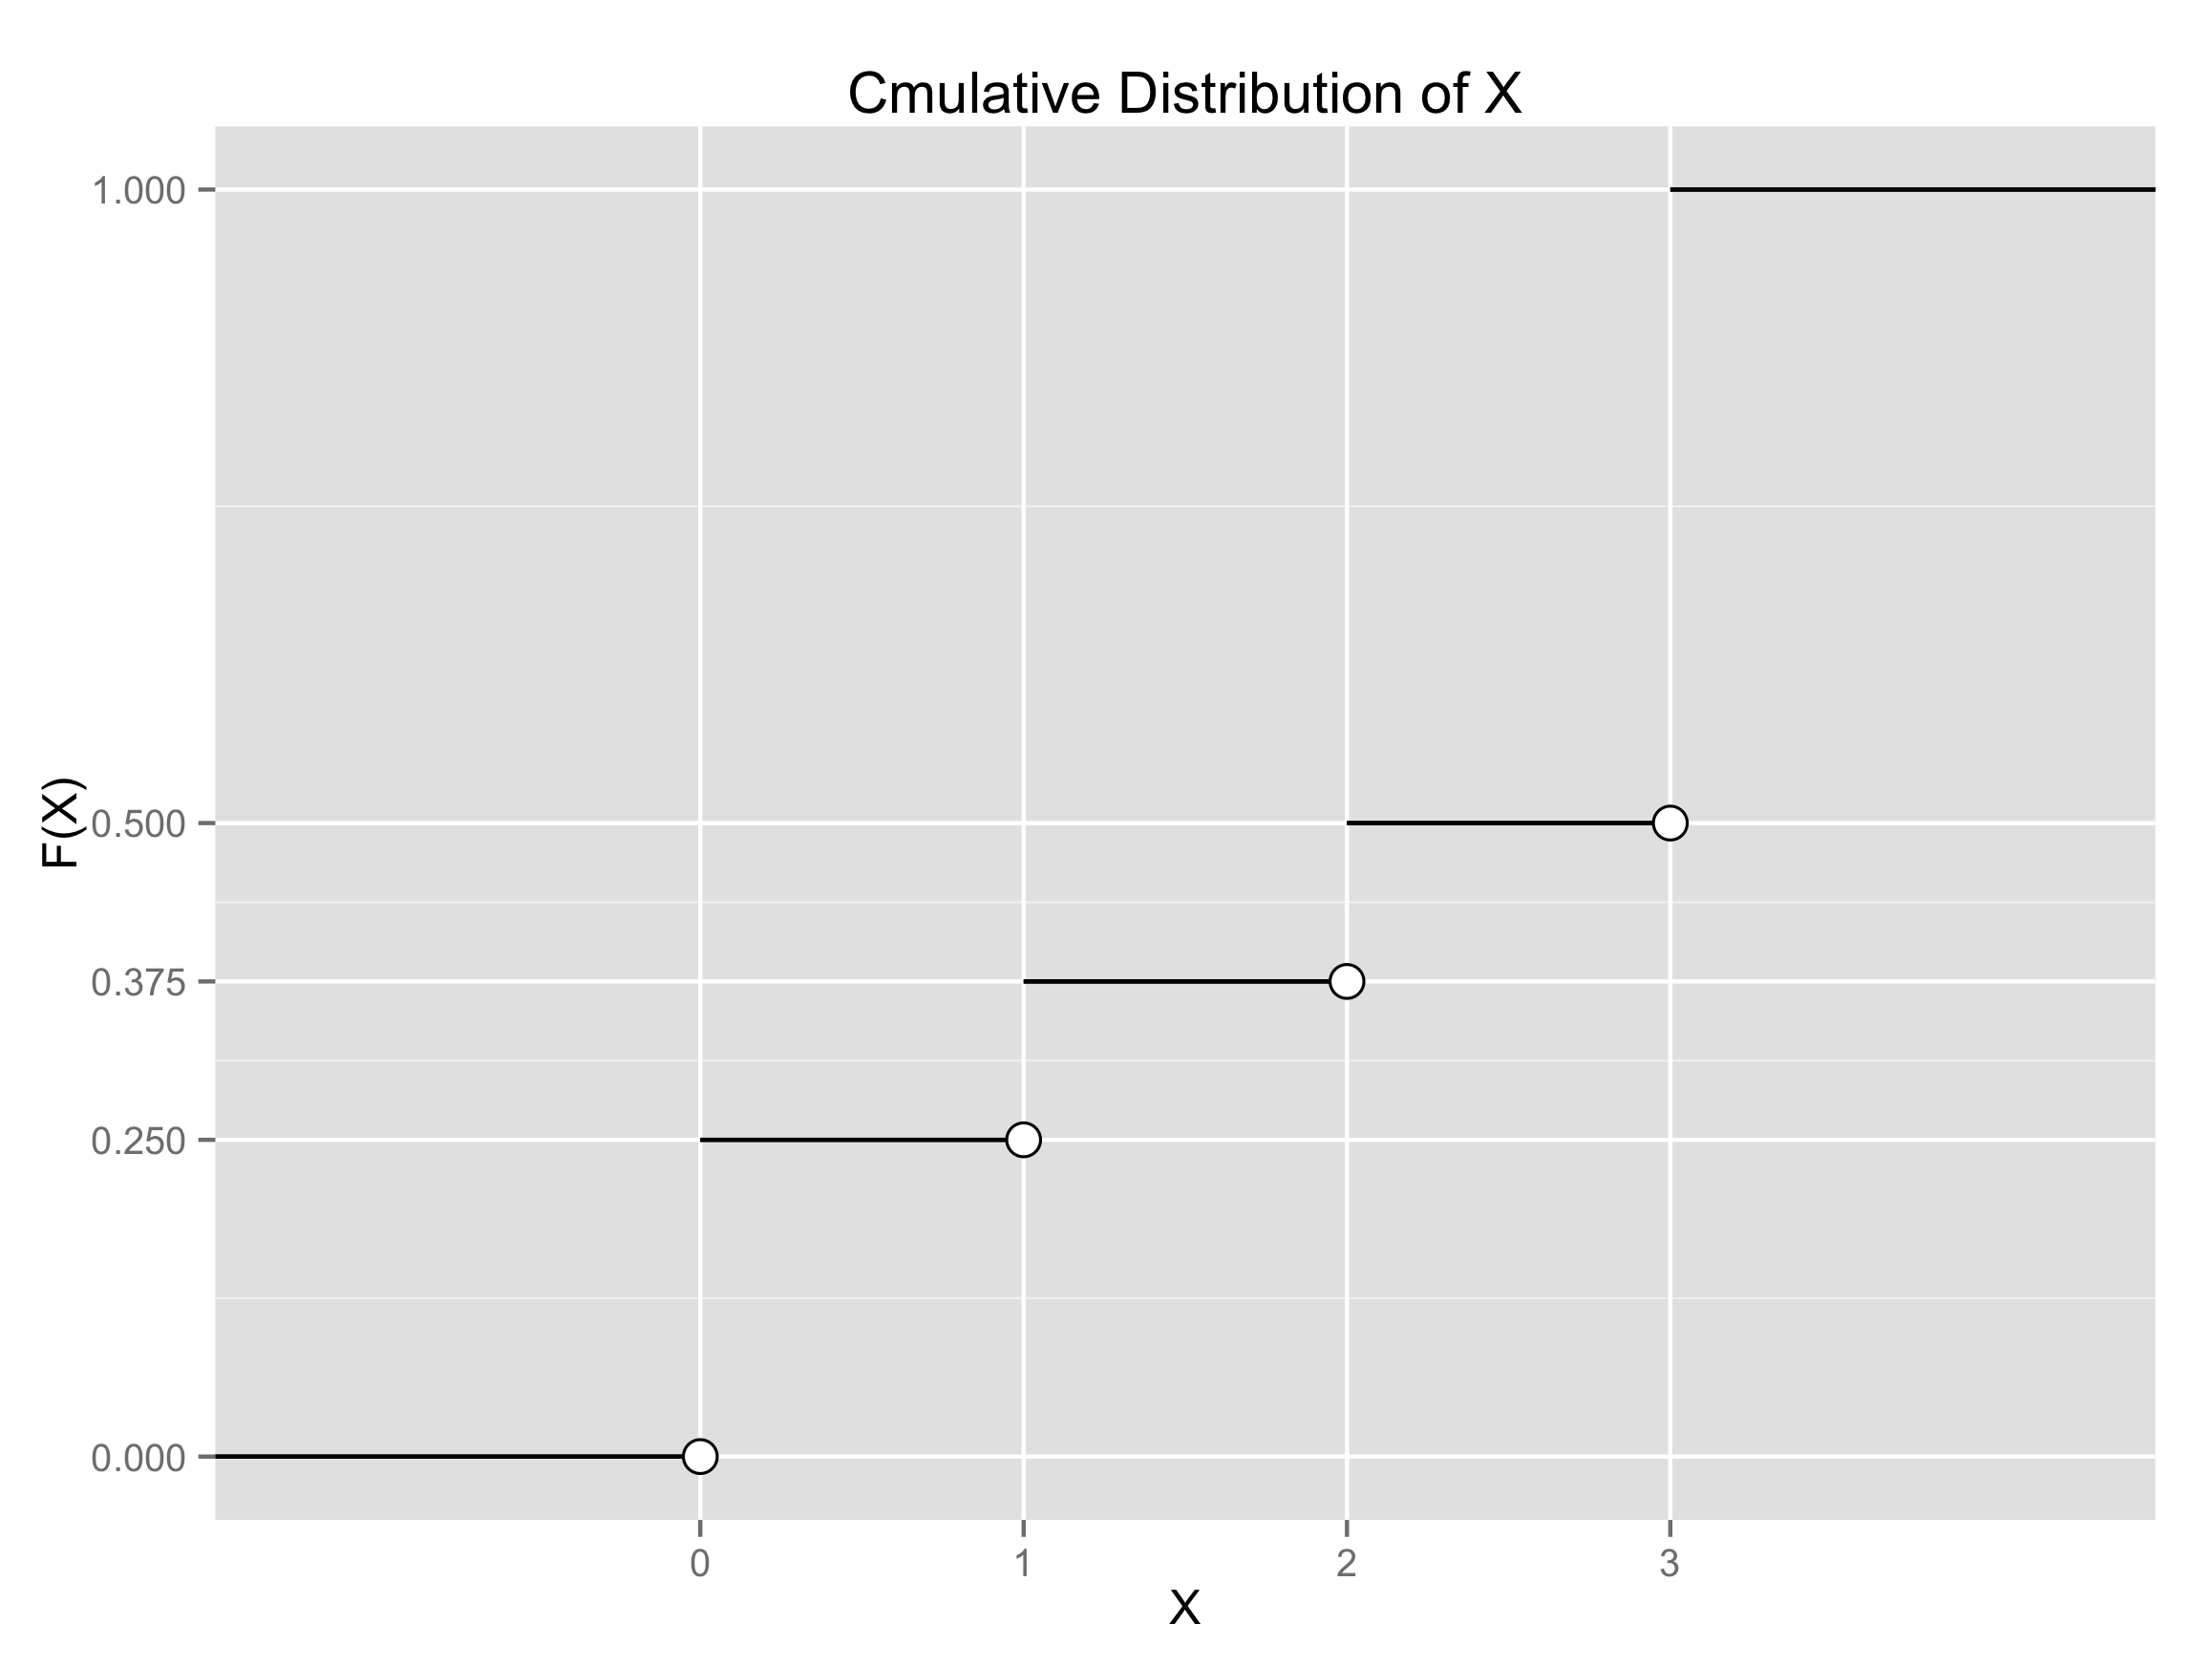
\includegraphics[width=10cm, height=8cm]{cdf_plot}
\end{center}


\bigskip
\bigskip
 %%%%%%%% Question 2 %%%%%%%%%
\begin{question}{2.2} A certain type of cancer is known to be present in 2 percent of the population of males in their fifties.
A test for the disease is advertised by a pharmaceutical company to be 3\% false negative and 1\% false positive.
\begin{enumerate}
\item{ Compute the probability that you have cancer if you are tested positive.}
\item{To make sure that you really have cancer an invasive and expensive surgery is needed. Your health insurance company is not willing to pay for this unless the pharmaceutical company improves its test in such way that that at least 90\% of people who are tested positive actually have the disease. How low should be the rate of false positive for the test to reach this goal? (Assume that the rate of false negative remains the same).}
\end{enumerate}

\end{question}

 \textbf{\color{TealBlue}\emph{Answer:} } 
 We'll use the following notation for the given data:
 \begin{itemize}
   \item The probability of the disease being present in the population of males over fifty: $P(D) = .02$. (Thus 98\% of this population is disease-free: $P(D^c) = .98$.)
  \item The probability of the test indicating that there is \emph{no disease} when in fact the disease is present (false negative): $P(T\text{--} \mid  D) = .03$. (Thus the probability of a \emph{true positive}, i.e. the test indicating that there \emph{is} disease when in fact the disease is present, $P(T\text{+} \mid  D)$, is then 97\%.)
  \item The probability of the test indicating that there is \emph{disease} when the disease is \emph{not} present (false positive): $P(T\text{+} \mid  D^c) = .01$
  \item We would like the probability $P(D \mid  T\text{+})$ of a person having the decease when the test result is positive to be at least 90\%. 
\end{itemize}

By Bayes' rule, the probability of the disease being present when the test indicates that it is present is:
 \begin{align*}
P(D \mid T\text{+}) = \frac{P(T\text{+} \mid  D) P(D) } {P(T\text{+} )} 
&= \frac{P(T\text{+} \mid  D) P(D) } {P(T\text{+} \mid  D) P(D) + P(T\text{+} \mid  D^c) P(D^c) } \\
&= \frac{.97 \times .02 } {.97 \times .02 + .01 \times .98} \\
&= 0.664
\end{align*}

 We would like to increase this probability from 66\% to at least 90\% by decreasing the probability of the false positives. That is, we would like to make the $P(T\text{+} | D^c)$ term in the denominator smaller. So let's solve the following inequality for $x$:
 \begin{align*}
 .9 &< \frac{.97 \times .02}{.97 \times .02 + x\times .98}\\
 .9 &< \frac{.0194} { .0194 +  .98x}\\
\end{align*}
 \begin{align*} 
.01746 + .882 x &<  .0194 \\
.882 x &< .00194 \\
x &< 0.002199546
\end{align*}

Thus, the false positive rate should be smaller than about \emph{two in a thousand.}


\bigskip
\bigskip
 %%%%%%%% Question 3 %%%%%%%%%
\begin{question}{2.3} Suppose there is a continuous random variable $X$ with \texttt{cdf} $F(x) $. Let $ Y = F(X) $. What is the distribution of $Y$? 
\end{question}

\textbf{\color{TealBlue}\emph{Answer:} } 
First, we note that the domain of the \texttt{r.v.}$Y$ is $[0, 1]$ Also, if $F(X)$ is a monotonically increasing function, it has a unique inverse, and we can write: 


$$
P ( Y \leq y ) = P( F(X) \leq y) = P( X \leq F^{-1}(y) ) = y
$$

That is, $Y$ has to be uniformly distributed over $[0, 1]$: $Y \sim U[0, 1]$.


\bigskip
\bigskip
 %%%%%%%% Question 4 %%%%%%%%%
\begin{question}{2.4} 
Generate 10,000 random samples from a distribution with the \texttt{pdf} $f(x) = 3 x^2 1(0 < x < 1) $. State your steps and program it in \texttt{R}. After generating these random numbers, plot its density and compare it with the actual pdf function. (Hint: Use the result from Problem 3.)

\end{question}


\textbf{\color{TealBlue}\emph{Answer:} } To generate random samples from a distribution with the \texttt{pdf} $f(x) = 3 x^2 1(0 < x < 1) $, we 

\begin{enumerate}
\item Compute the \texttt{cdf} of $X$, $F(X)$. This is simply $u = F(x) = x^3$ on the interval from $[0,1]$ ( and it's $1$ whenever $x \geq 1$ and $0$ whenever $x \leq 0$)
\item Then find its inverse: $F^{-1}(u) = u^{1/3}$ (where $u$ ranges from $0$ to $1$)
\item Finally, we generate uniform \texttt{r.v.}s and transform them with this $F^{-1}$ to obtain the needed samples
\end{enumerate} 
 The \texttt{R} code that performs the above steps and generates the figures below can be found at \url{https://github.com/david-dobor/8003/blob/master/week2/q4hw1.R} 
 

 \begin{center}
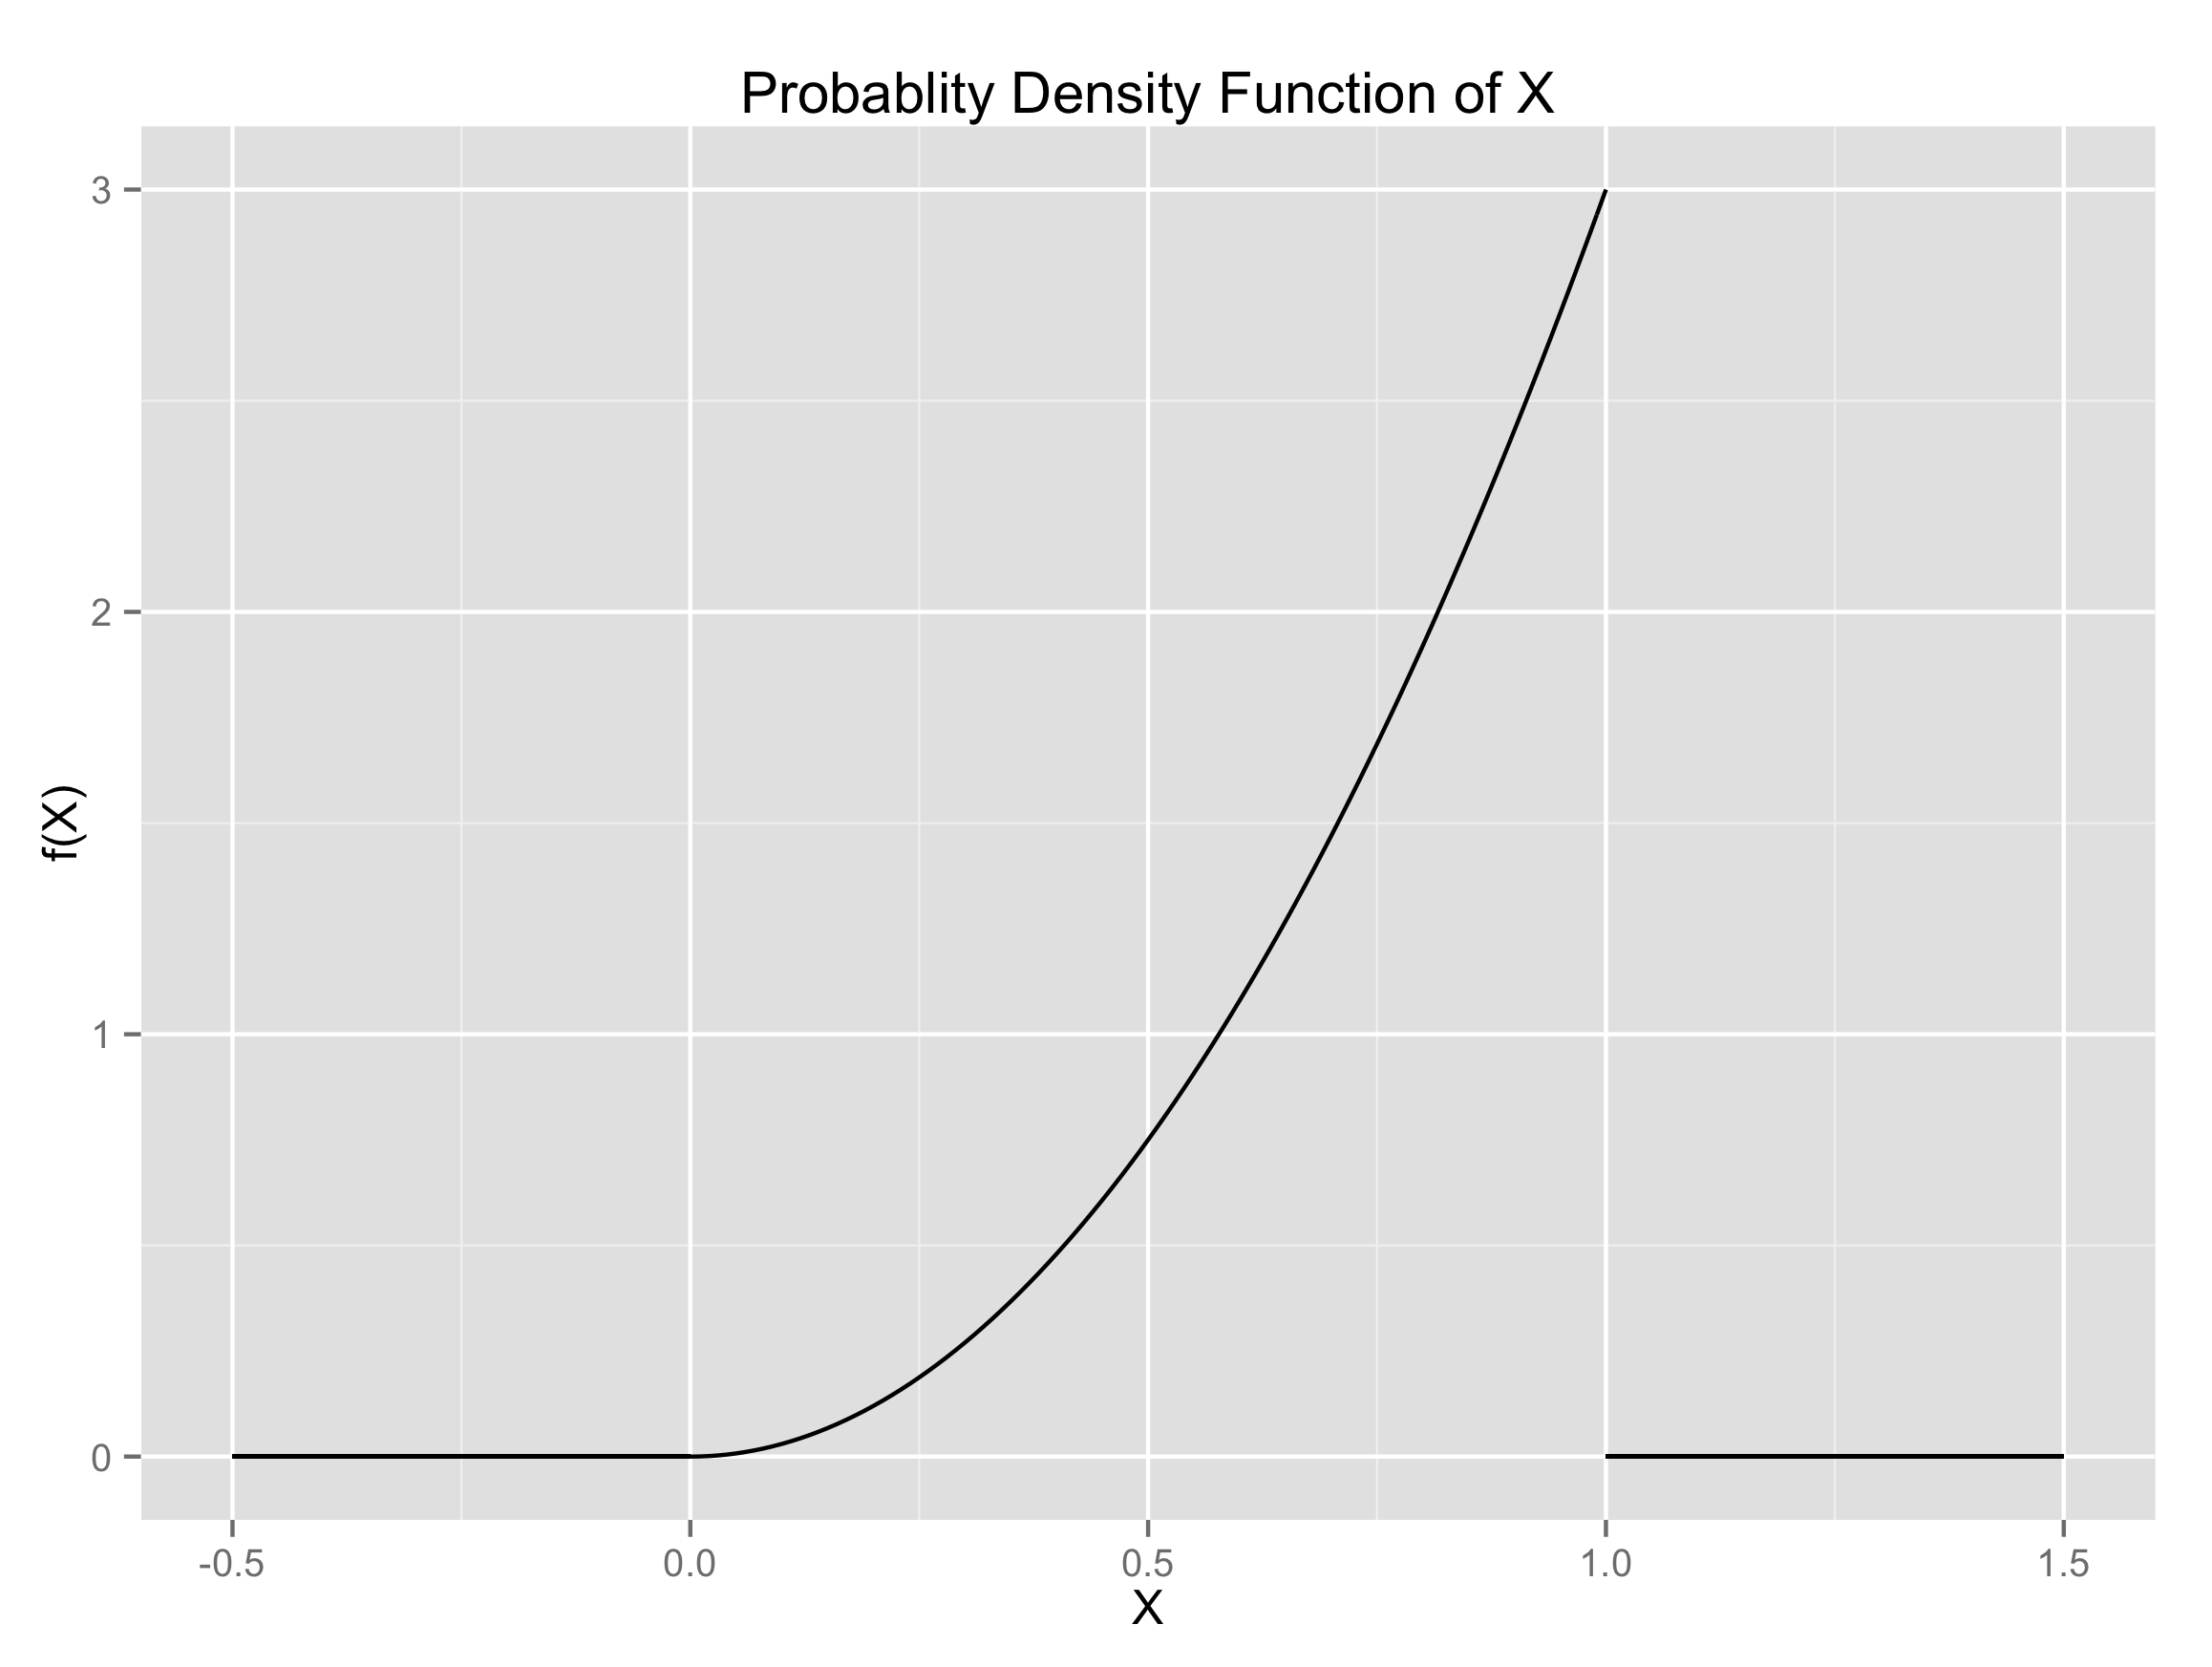
\includegraphics[width=10cm, height=8cm]{density}
\end{center}
 
 \begin{center}
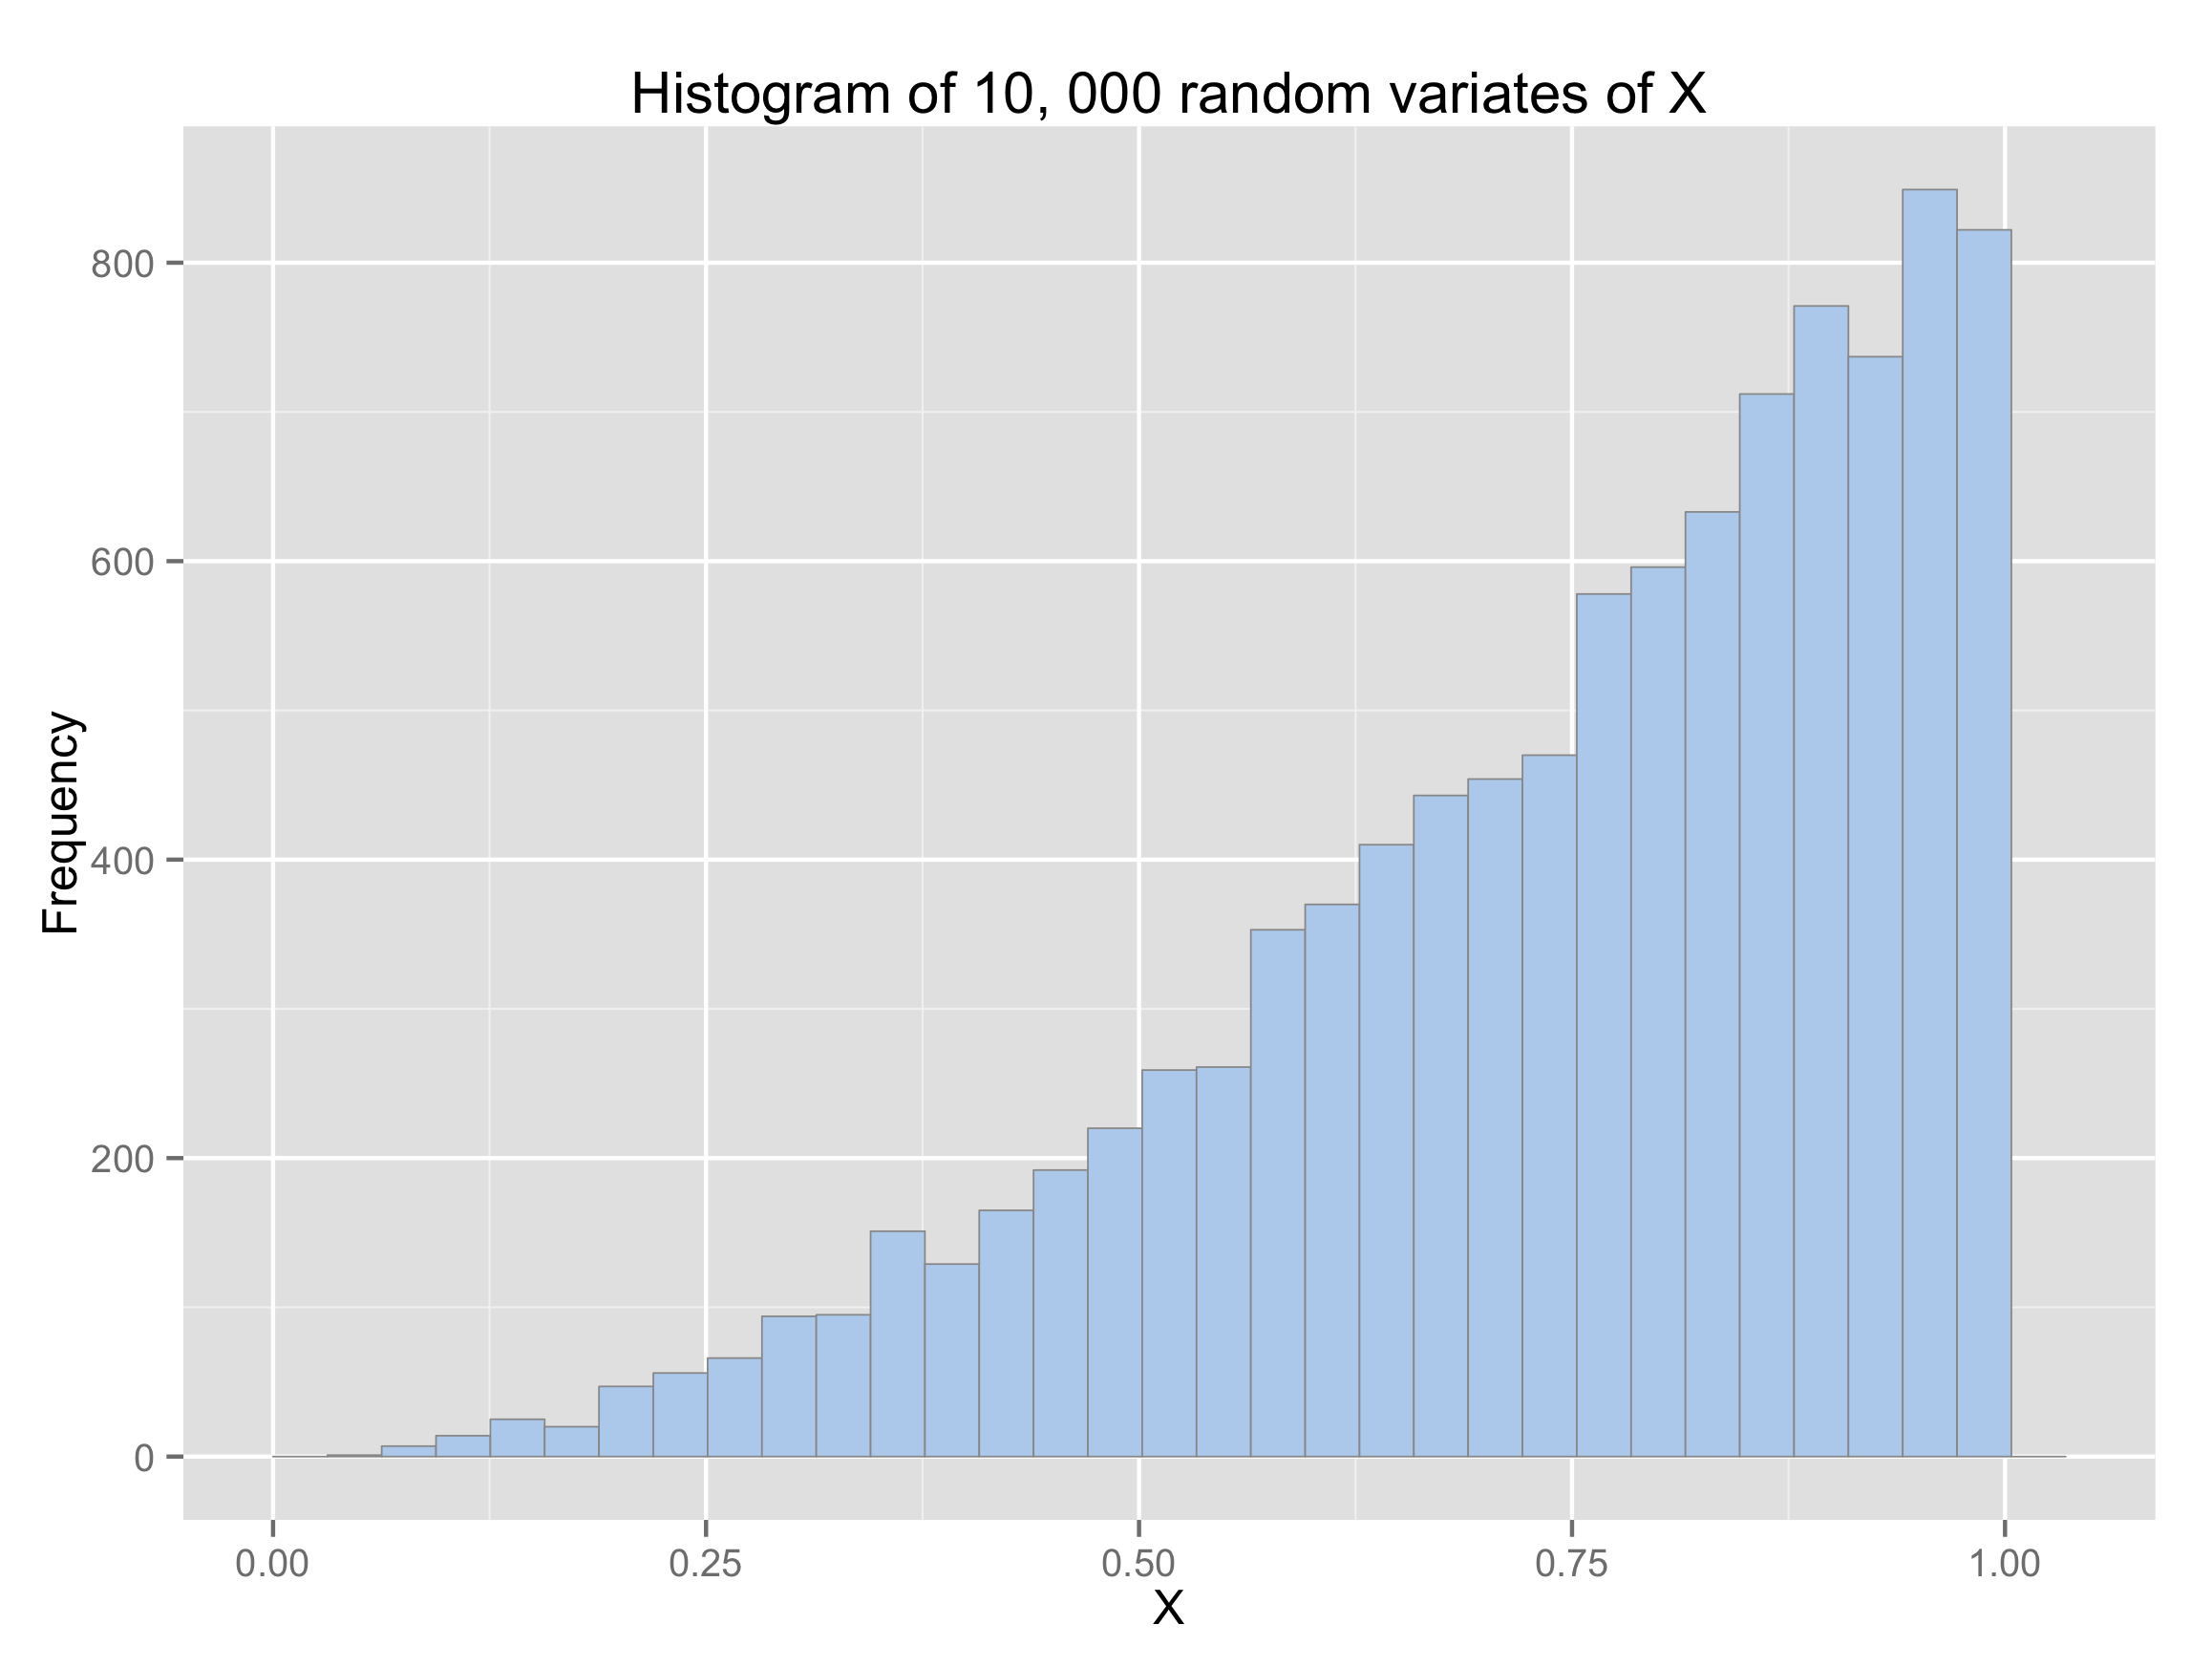
\includegraphics[width=10cm, height=8cm]{histogram}
\end{center}

\end{document}
%Note 1: The * tells LaTeX not to number the lines.  If you remove the *, be sure to remove it below, too.
%Note 2: Inside the  environment, you do not want to use $-signs.  The reason for this is that this is already a math environment. This is why we have to include \text{} around any text inside the align environment.

%\begin{proof}
%Blah, blah, blah.  
%\end{proof}

